\documentclass[11pt,a4paper]{article}
%%%%%%%%%%%%%%%%%%%%%%%%%%%%%%%%%%%%%%%%%%%%%%%%%%%%%%%%
%                      PACKAGES                        %
%%%%%%%%%%%%%%%%%%%%%%%%%%%%%%%%%%%%%%%%%%%%%%%%%%%%%%%%

\usepackage[utf8]{inputenc}
\usepackage{graphicx} % Allows you to insert figures
\usepackage[export]{adjustbox}
\usepackage{booktabs}
\usepackage{amsmath} % Allows you to do equations
\usepackage{helvet}
\usepackage{hyperref}
\renewcommand{\familydefault}{\sfdefault}
\usepackage[a4paper, total={6.5in, 9.5in}]{geometry} % Formats the paper size, orientation, and margins
\linespread{1.1} % about 1.5 spacing in Word
\setlength{\parindent}{0pt} % no paragraph indents
\setlength{\parskip}{1em} % paragraphs separated by one line
\usepackage{listings}
\usepackage{enumitem}
\usepackage{xcolor}
\usepackage{hyperref}
\hypersetup{
	colorlinks=true,
	urlcolor=cyan,
	linktoc=none,
}
\usepackage{fancyhdr}
\pagestyle{fancy}
\fancyhead[L,C,R]{}
\fancyfoot[L]{Occupi - Office Capacity Predictor}
\fancyfoot[C]{}
\fancyfoot[R]{\textbf{\thepage}}
\renewcommand{\headrulewidth}{0pt}
\renewcommand{\footrulewidth}{0.5pt}

\definecolor{codegreen}{rgb}{0,0.6,0}
\definecolor{codegray}{rgb}{0.5,0.5,0.5}
\definecolor{codepurple}{rgb}{0.58,0,0.82}
\definecolor{backcolour}{rgb}{0.95,0.95,0.92}

\lstdefinestyle{mystyle}{
backgroundcolor=\color{backcolour},
commentstyle=\color{codegreen},
keywordstyle=\color{magenta},
numberstyle=\tiny\color{codegray},
stringstyle=\color{codepurple},
basicstyle=\ttfamily\footnotesize,
breakatwhitespace=false,
breaklines=true,
keepspaces=true,
numbers=left,
numbersep=5pt,
showspaces=false,
showstringspaces=false,
showtabs=false,
tabsize=2,
}

\lstset{style=mystyle}
\def\code#1{\texttt{#1}}

%%%%%%%%%%%%%%%%%%%%%%%%%%%%%%%%%%%%%%%%%%%%%%%%%%%%%%%%
%            TITLE PAGE & TABLE OF CONTENTS            %
%%%%%%%%%%%%%%%%%%%%%%%%%%%%%%%%%%%%%%%%%%%%%%%%%%%%%%%%

\begin{document}
\begin{titlepage}
    \centering
    
\includegraphics[width=0.4\textwidth]{logo-white.png}\par\vspace{1cm}
    {\scshape\LARGE Data Science: Innovative use of data \par}
    \vspace{1.5cm}
    {\huge\bfseries Occupi - Office Capacity Predictor\par}
    \vspace{2.5cm}
    \begin{tabular}{|c|c|}
        \hline
        \textbf{Name}      & \textbf{Student Number} \\
        \hline
        Rethakgetse Manaka & u22491032               \\
        Kamogelo Moeketse  & u22623478               \\
        Michael Chinyama   & u21546551               \\
        Tinashe Austin     & u21564176               \\
        Carey Mokou        & u21631532               \\
        \hline
    \end{tabular}
    \vfill
    {\large October 10, 2024\par}
\end{titlepage}

\tableofcontents
\pagebreak

%%%%%%%%%%%%%%%%%%%%%%%%%%%%%%%%%%%%%%%%%%%%%%%%%%%%%%%%
%                MAIN DOCUMENT CONTENT                 %
%%%%%%%%%%%%%%%%%%%%%%%%%%%%%%%%%%%%%%%%%%%%%%%%%%%%%%%%

\section*{Introduction}
\addcontentsline{toc}{section}{Introduction}
During the development of Occupi, a strong foundation of data science principles and methodologies was established to ensure that the project would deliver high-impact insights 
and predictions. This project was built with the primary goal of handling sequential data efficiently using a mixture of Convolutional Neural Networks (CNN) 
and Long Short-Term Memory (LSTM) networks for time series data classification. 
Additionally, MongoDB functions and triggers were employed to handle real-time user statistics and data collection.

The integration of CNN and LSTM models allowed us to capture both spatial and temporal dependencies in the data, 
ensuring accurate predictions and classifications. CNNs were used to extract features from the raw time series data, 
while LSTMs captured long-term dependencies, making the model particularly effective for time series classification. 
This hybrid approach enabled our system to handle large datasets efficiently and provided meaningful predictions in areas such as capacity prediction.

In addition to the machine learning models, MongoDB functions, aggregation, and triggers were crucial for automating the processing of user data and generating statistics in real time. 
This streamlined the data pipeline, ensuring that the latest data was always available for analysis, thus maintaining the accuracy and relevance of the user statistics.

\pagebreak

\section*{Data generation and Model Training}
\addcontentsline{toc}{section}{Data generation and Model Training}
The use of Mockaroo and VBA was instrumental in simulating office attendance data that reflected real-world trends under various conditions, such as public holidays, weekends, and peak hours. 
This simulated data was essential in generating large, high-quality datasets that were representative of the diverse scenarios that our predictive models would encounter. 
This foundation allowed us to begin the initial stages of model training with confidence, knowing that the datasets were comprehensive and varied.

\begin{figure}[htbp]
    \centering
    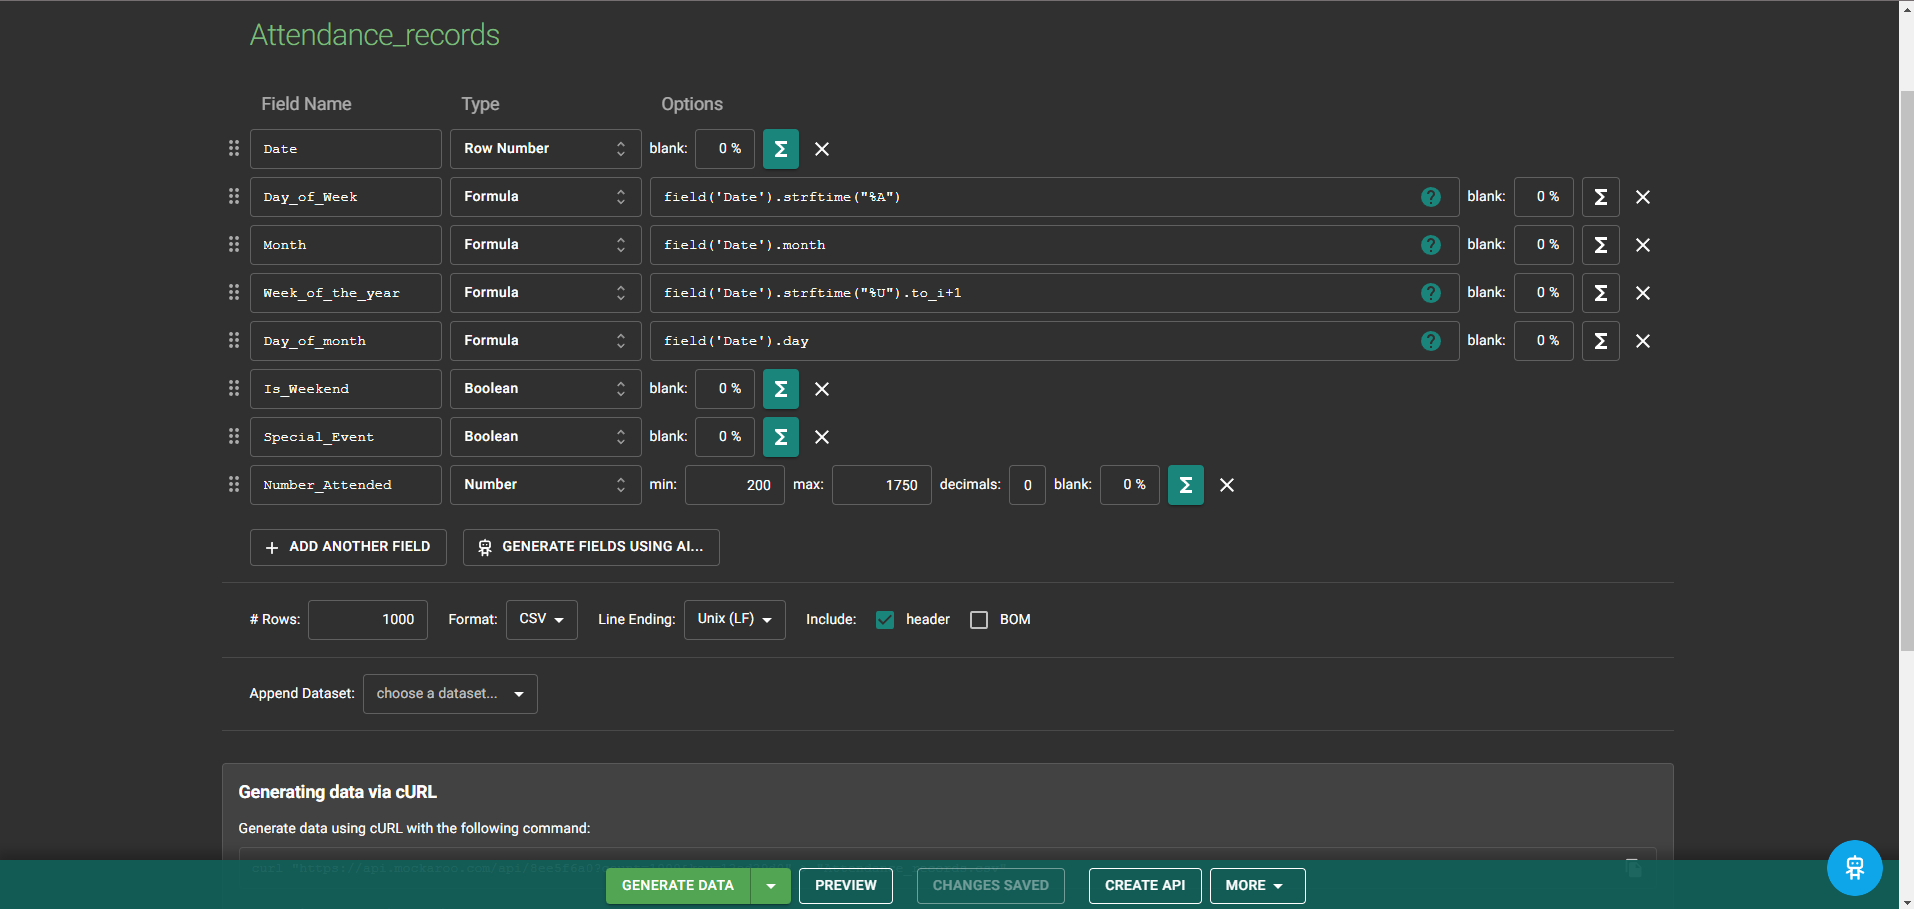
\includegraphics[width=0.9\textwidth]{Mockaroo.png}
\end{figure}

To handle the sequential nature of this data, we employed a mixture of Convolutional Neural Networks (CNNs) and Long Short-Term Memory (LSTM) networks. 
The CNNs were responsible for extracting features from the raw time series data, capturing patterns in attendance fluctuations, 
while the LSTMs processed the temporal dependencies, enabling the model to learn from the historical trends and make accurate future predictions.

\subsection*{Iterative Training and Optimization}
Once the initial models were trained on the simulated data, we rigorously evaluated their performance based on accuracy, precision, recall, 
and other relevant metrics. 
Our target was to achieve a model accuracy of at least 70\%, 
which we identified as the threshold for reliable predictions in real-world applications. 
However, the first few iterations of model training showed that while the models captured some patterns, the accuracy was still below our desired threshold.

To address this, we adopted an iterative approach to model training and optimization. This process involved the following steps:

\subsubsection*{Hyperparameter Tuning}
We adjusted key hyperparameters such as learning rate, batch size, and the number of epochs. 
By experimenting with different combinations of these parameters, we gradually improved the performance of our models. 
Grid search and random search techniques were employed to find the best hyperparameter settings for both the CNN and LSTM components of the model.

\subsubsection*{Data Augmentation and Feature Engineering}
We further enhanced the datasets by introducing additional features that could improve the model's ability to make predictions. These features included:
\begin{itemize}
    \item \textbf{Predicted Class}: To easily classify attendance levels.
    \item \textbf{Predicted Level}: To capture ranges of attendance, such as low, medium, and high.
\end{itemize}

\subsubsection*{Regularization Techniques}
To prevent overfitting during training, we applied techniques such as dropout in the LSTM layers, which randomly deactivates certain neurons during training. 
This forced the model to learn more generalized patterns and improved its performance on unseen data. 
Additionally, L2 regularization was applied to penalize excessively large weights, encouraging the model to focus on the most relevant features.

\subsection*{Achieving 70\%+ Accuracy}
Through this iterative process of training, evaluation, and optimization, we were able to consistently improve the performance of our models. 
After several rounds of refinement, the CNN-LSTM hybrid model achieved an accuracy above 70\%. 
This threshold was met by balancing the complexity of the model with its ability to generalize across diverse office attendance scenarios, 
ultimately resulting in a model capable of making reliable predictions on real-world data.

\begin{figure}[htbp]
    \centering
    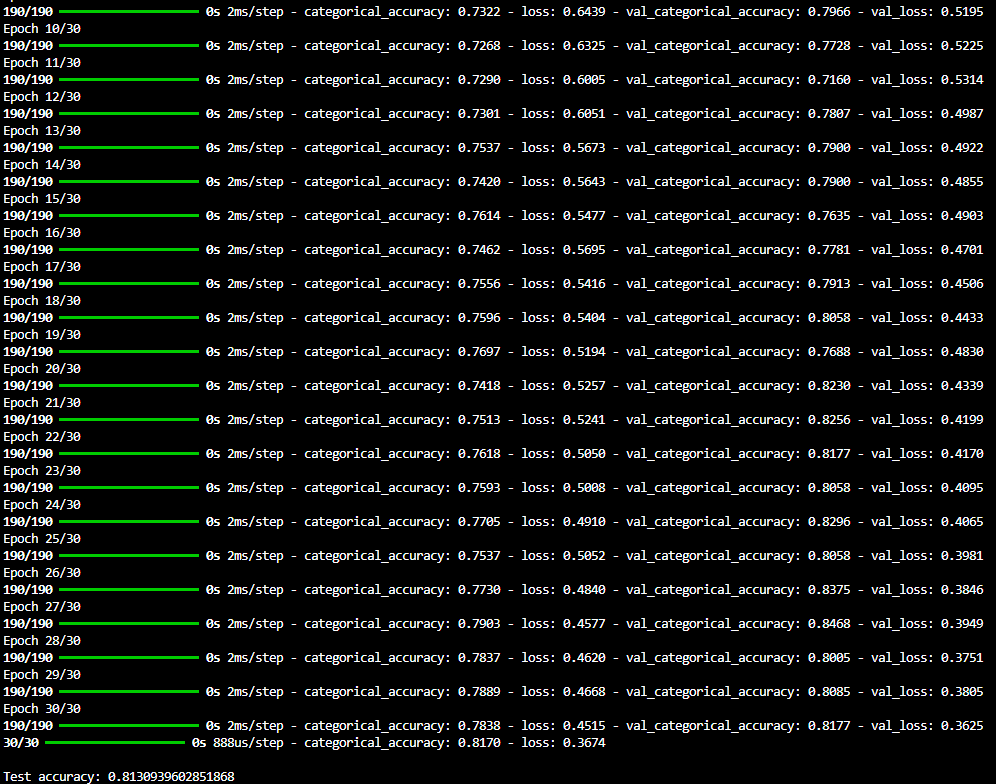
\includegraphics[width=0.9\textwidth]{Training.png}
\end{figure}

\subsection*{Prediction and Reporting}
The model was used to generate predictions for both hourly and daily office attendance. 
These predictions proved valuable in producing detailed reports for capacity predictions, allowing stakeholders to make informed decisions about space utilization. 
By predicting attendance levels on an hourly and daily basis, the system provided actionable insights into peak times, potential under-utilization, and how attendance varied throughout the week.

These reports allowed for:
\begin{itemize}
    \item \textbf{Hourly Predictions}: Managers could monitor expected attendance levels hour-by-hour, helping them plan resources, staffing, and space requirements effectively.
    \item \textbf{Daily Predictions}: Daily predictions provided a broader view of office occupancy trends, allowing for better scheduling, event planning, and overall space management.
\end{itemize}

The combination of accurate predictions and detailed reporting helped stakeholders 
improve decision-making processes related to office capacity management, 
ensuring that both resources and spaces were optimally used. The predictions were visualized through graphs and dashboards, 
offering a clear and accessible view of expected attendance for any given time period.

\begin{figure}[htbp]
    \centering
    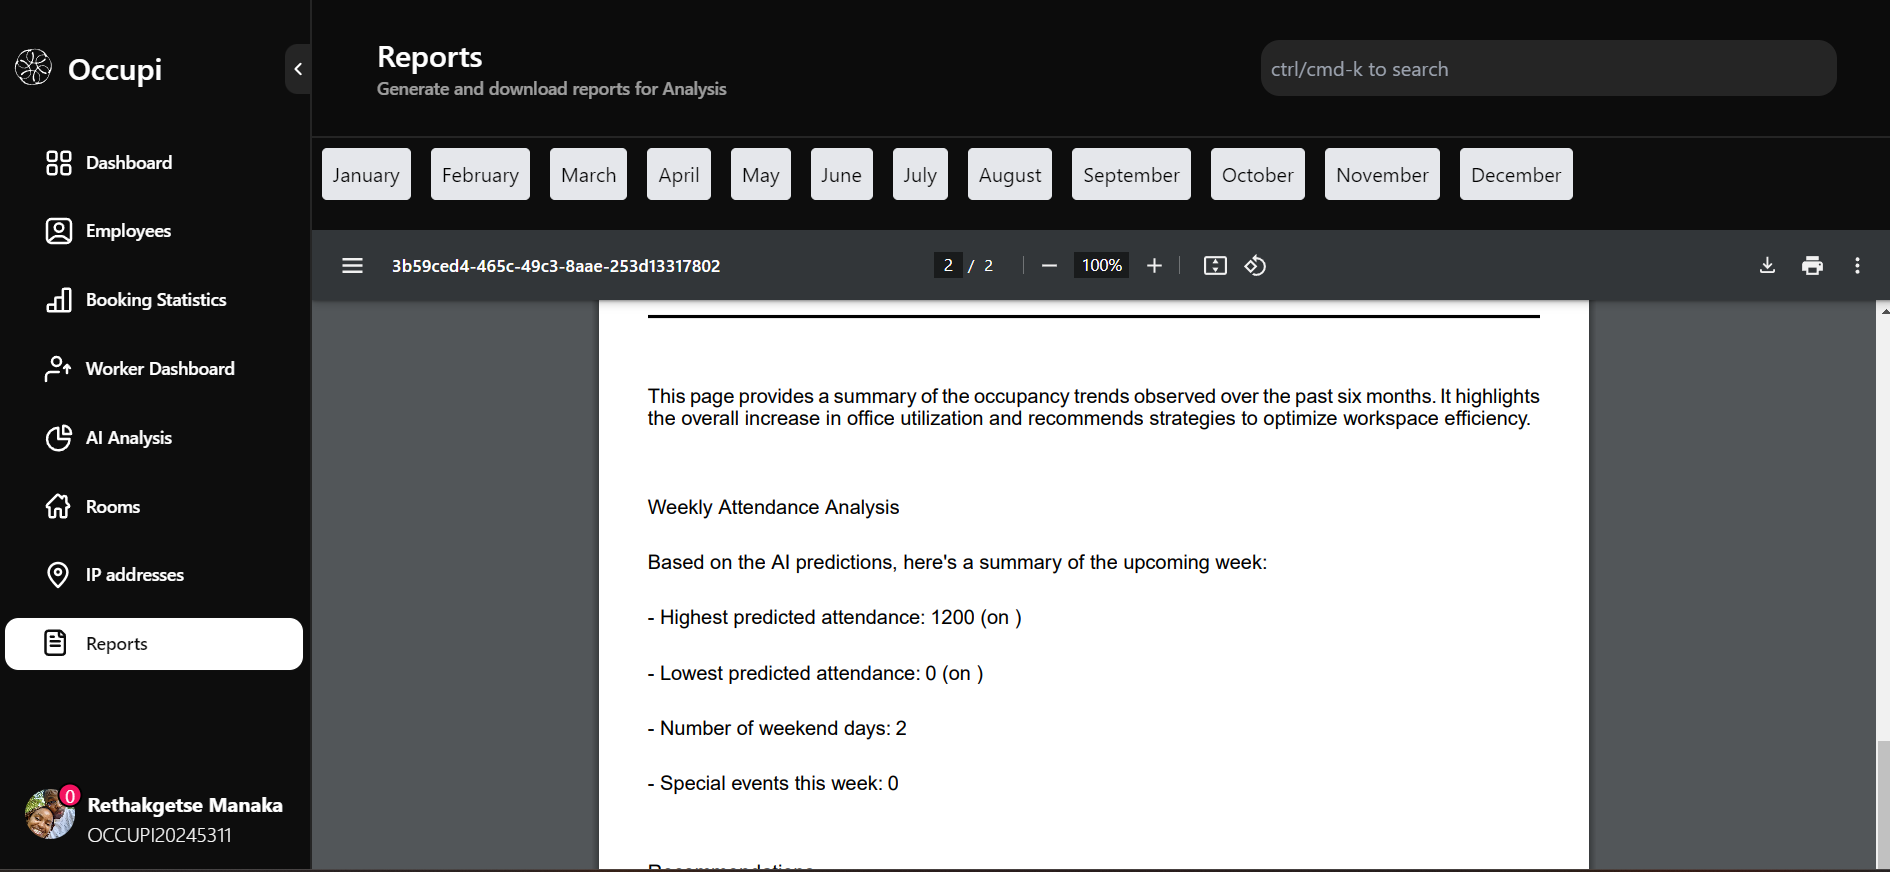
\includegraphics[width=0.9\textwidth]{Reports.png}
\end{figure}

\section*{MongoDB for User Statistics Processing}
\addcontentsline{toc}{section}{MongoDB for User Statistics Processing}

MongoDB played a critical role in processing user statistics by leveraging its powerful aggregation framework and triggers. 
The user statistics data was collected and stored in MongoDB, 
allowing us to generate real-time insights regarding work patterns, arrival and departure times, daily hours worked, and peak office hours.

\subsection*{Data Aggregation}
MongoDB's aggregation pipeline enabled us to efficiently process large volumes of data. Using the pipeline, we could:
\begin{itemize}
    \item \textbf{Calculate In-Office Rate}: The \texttt{CalculateInOfficeRate} function used the aggregation pipeline to compute the work ratio for each day of the week. 
    By grouping the data by weekday and calculating the in-office rate using the difference between entry and exit times, we could measure the attendance ratio.
    
    \item \textbf{Analyze Arrival and Departure Times}: The \texttt{AverageArrivalAndDepartureTimesByWeekday} function derived the average arrival and departure times using MongoDB’s 
    aggregation operators like \texttt{\$avg}. The \texttt{\$group} stage was used to calculate averages for each weekday, providing insights into workday start and end times.
    
    \item \textbf{Identify Peak Office Hours}: The \texttt{BusiestHoursByWeekday} function identified the top 3 busiest hours for each weekday by analyzing the 
    number of hours spent by users in the office. The data was grouped by weekday and hour to find peak attendance times, allowing managers to optimize resources.
\end{itemize}

\begin{figure}[htbp]
    \centering
    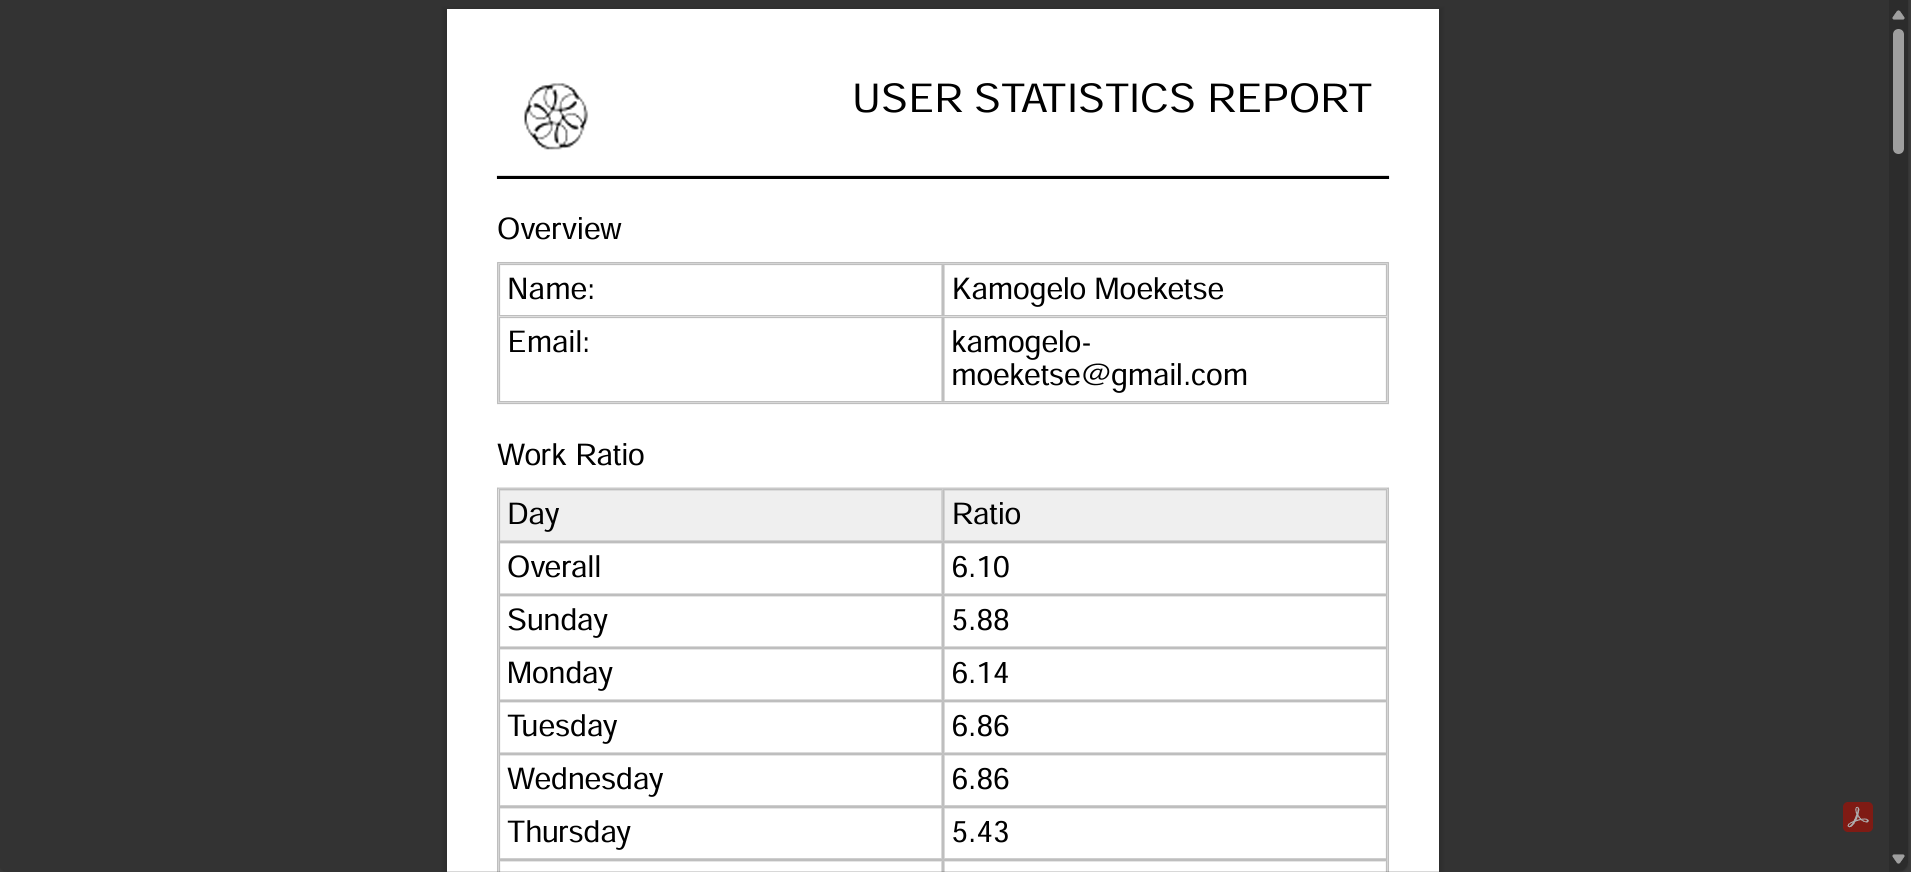
\includegraphics[width=0.9\textwidth]{User_Reports.png}
\end{figure}

\subsection*{Real-Time Triggers}
In addition to the aggregation framework, MongoDB triggers were employed to ensure that user statistics were continuously updated in real-time. 
This allowed us to capture live data as it was added to the database, automatically processing new entries without manual intervention. Triggers were used to:
\begin{itemize}
    \item \textbf{Update Daily Hours}: When new attendance data was added, triggers automatically calculated and updated the total hours worked for that day. 
    This ensured that reports were always up-to-date and reflected the latest available data.
    
    \item \textbf{Real-Time User Statistics}: Triggers calculated the total hours worked by each user based on their check-in and check-out times. 
    The calculated data was updated in real-time, providing immediate insights into user behavior.
\end{itemize}

By utilizing MongoDB's real-time processing capabilities and data aggregation pipelines, we were able to generate comprehensive reports and insights for user behavior. 
The statistics presented, such as the daily work ratios, arrival and departure times, and peak office hours, 
were all derived from the data stored in MongoDB and processed using these advanced features.

\pagebreak

\section*{Conclusion}
The integration of CNN and LSTM models, combined with extensive preprocessing, feature engineering, 
and real-time data collection using MongoDB functions and triggers, enabled us to build a highly effective system for predicting office attendance. 
Through continuous training and model refinement, we successfully achieved the project’s goal of delivering accurate, actionable insights.

\end{document}
